\subsection{RICH Detector}

The CLAS12 Ring Imaging Cherenkov Counter (RICH)~\cite{rich-nim} presently replaces one LTCC counter in the
Forward Detector (with a second RICH to be installed in the future replacing a second LTCC counter). When charged
particles traverse the aerogel radiator in the RICH volume, Cherenkov radiation is emitted with a characteristic cone
angle related to the particle velocity. These photons are distributed in a ring pattern that can be reconstructed by
collecting the photons using mirrors and PMTs (see Fig.~\ref{Fig:RayShow} for an example RICH event). The goal of
the RICH reconstruction is to provide an estimate of the Cherenkov angle for each detected photon and intercepted
particle track, to allow subsequent particle identification. This requires input from the Forward Detector tracking
service, which defines the trajectory of particle tracks inside the detector and, in particular, the track intersection
point and direction within the aerogel radiator and the photodetector plane composed of multi-anode PMTs (MaMPTs).

\begin{figure}[t]
\begin{center}
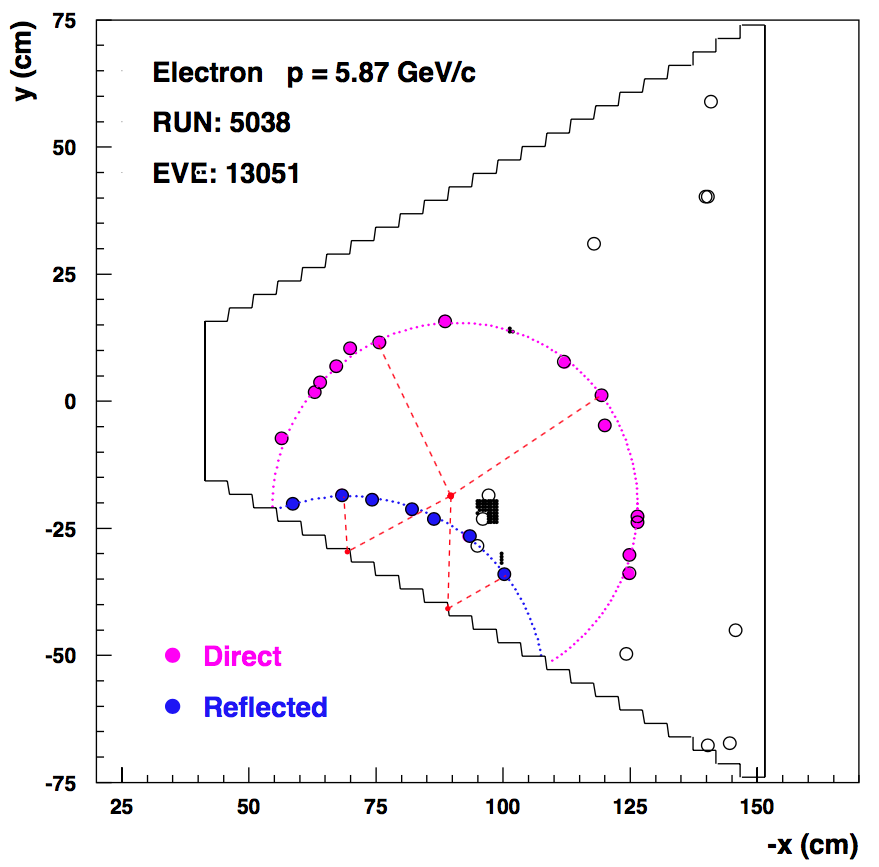
\includegraphics[width=0.8\columnwidth]{pics/example.png}
\end{center}
\caption{Example of a reconstructed RICH event from beam data. Small points indicate the trial pattern expected
  for an electron, as identified by CLAS12. The dashed lines show examples of ray-traced photon paths from the
  common emission point (in the radiator) to the detected hit: two direct photons emitted upwards and two reflected
  photons emitted downwards. The open circles are the detected RICH hits. The circles are filled in the case that a
  viable traced solution has been found. The central cluster is generated by the track impact on the MaPMT plane.}
\label{Fig:RayShow}
\end{figure}

In the first phase, the RICH reconstruction identifies the cluster of hits produced by the charged particle in the
sensor plane. In the second phase, the cross-talk signals are identified by means of an amplitude analysis (based on
the time-over-threshold information) in conjunction with geometrical constraints, taking into account that a cross-talk
hit should be in the proximity of a genuine hit. Finally, hits neither belonging to a cluster nor flagged as cross-talk are
considered as Cherenkov photon candidates. 

The photon path inside the RICH is reconstructed in two complementary ways, taking the middle point of the hadron
trajectory inside the radiator as the emission point, and the hit pixel coordinates as the detection point. The first
method uses an analytic formula that takes into account the refraction at the aerogel face and is only valid for directly
detected photons. It provides an exact solution. The second method uses a ray-tracing algorithm that also takes into
account the mirror reflections. It provides a numeric solution based on an iterative procedure. Both methods return the
reconstructed Cherenkov angle in conjunction with the corresponding aerogel refractive index, which can vary slightly
with respect to the nominal value due to the chromatic dependence on the unknown photon energy.

The relevant RICH components (aerogel, mirrors, MaPMT plane) are converted into ray-tracing planes or spheres
where the photon can undergo refraction, reflection, or detection. Each ray-tracing element can be independently
aligned. The alignment procedure uses as a benchmark the Cherenkov signal generated by electrons, as identified
by the HTCC and ECAL. For these particles, the expected Cherenkov angle is given by the known particle momentum
(from DC tracking) and mass. The position and orientation of the MaPMT plane is defined by minimizing the average
distance that matches the RICH clusters to the charged tracks extrapolated to the MaPMT plane. Any other RICH
component can be aligned with respect to the MaPMT plane by selecting the sub-sample of photons passing through
that component. The alignment is done by minimizing the average distance between the ray-traced detection point
(RdP) and the corresponding measured MaPMT hit over the selected sub-sample of photons.

For each hadron track, the ray-tracing algorithm progresses as described in the following. A trial photon is a
hypothetical photon assumed to originate from the emission point at a Cherenkov angle $\theta_T$ and an azimuthal
angle $\phi_T$, with the corresponding RdP $T(\theta_T, \phi_T)$ defined by the ray-tracing algorithm. A limited
ensemble (on the order of 100) of trials is initially traced having $\theta_T$ defined by a particle hypothesis, i.e.
electron for a particle identified as an electron in CLAS12, pion otherwise, and $\phi_T$ uniformly distributed around
the charged particle trajectory, see Fig.~\ref{Fig:RayShow}. For each MaPMT measured hit, the closest trial RdP is
taken to be the starting point of the iterative ray-tracing procedure for that hit.

To initiate the iterative procedure, the closest trial RdP is required to stay at a distance from the hit smaller than
10~cm, which is twice the typical distance between the initial trial RdPs on the MaPMT plane. At each step, the
closest trial is re-traced by varying its angles by the expected Cherenkov angle resolution $\sigma$ to define the
corresponding displaced RdPs $T_{\theta} (\theta_T + \sigma, \phi_T)$ and $T_{\phi}(\theta_T, \phi_T + \sigma)$.
The distance vectors $\overrightarrow{TT_\theta}$ and $\overrightarrow{TT_\phi}$, connecting each rotated trial
RdP to the initial trial RdP, naturally define a reference system in the MaPMT plane, see Fig.~\ref{Fig:RayAlgo}. The
distance vector $\overrightarrow{TH}$ between the measured hit $H$ and the closest trial RdP position $T$ is
projected onto the reference vectors to get an estimate of the next angular step. In particular, the scale factor
$f$ of the polar angle step $\Delta \theta = f \sigma$ is defined by projecting the distance vector
$\overrightarrow{TH}$ onto the reference vector $\overrightarrow{TT_\theta}$:
$f=(\overrightarrow{TH} \cdot \overrightarrow{TT_\theta}) / |\overrightarrow{TT_\theta}|^2$. The factor $f$ can
be either positive or negative, depending on if the rotated point moves toward or away from the measured hit. The
same is done for the azimuthal angle $\phi$. 

\begin{figure}[t]
\begin{center}
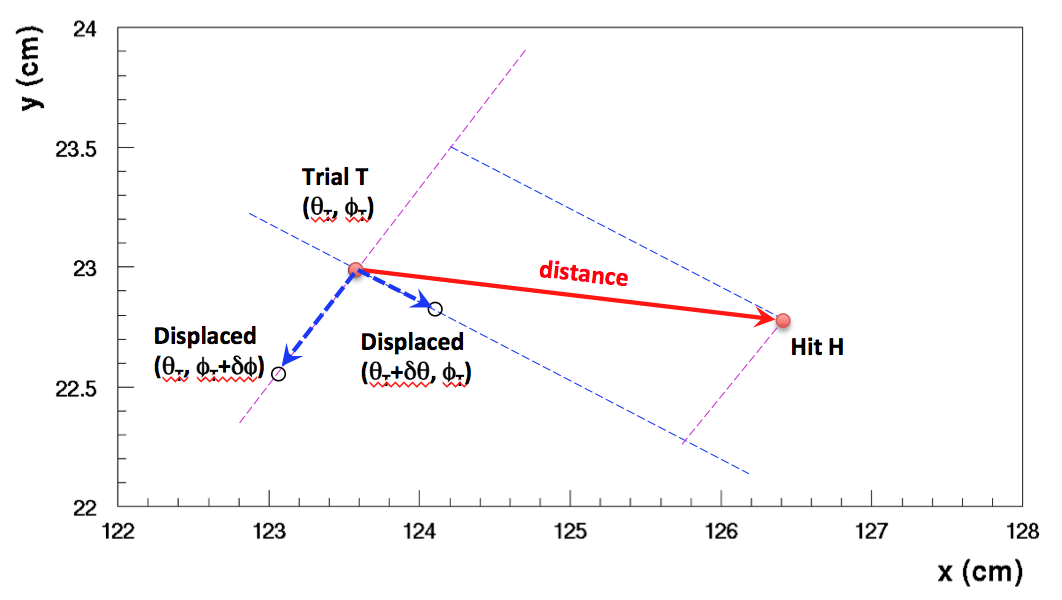
\includegraphics[width=1.0\columnwidth]{pics/ray_trace_example.png}
\end{center}
\caption{Example of iteration of the ray-tracing photon path reconstruction in the RICH $(x,y)$ plane. The emission
  polar $\theta_T$ and azimuthal $\phi_T$ angles of the closest trial photon are varied by the expected Cherenkov
  angle resolution $\sigma$ to extrapolate the corresponding displacements of the detection point. The distance
  between the measured and the trial hit is projected onto such displacements to quantify the next angular step in
  units of $\sigma$. See text for details.}
\label{Fig:RayAlgo}
\end{figure}

The angles of the trial photon are modified by the calculated $\Delta\theta$ and $\Delta\phi$ angular shifts,
and the procedure is repeated. At each step, the trial RdP gets closer to the measured hit, but an exact solution
cannot be found as the procedure uses a linear approximation relating the distances in the MaPMT plane with the
angular rotations in the 3D space. The iterative procedure stops when the distance of the trial RdP from the
measured hit is smaller than a fraction of the MaPMT pixel size, i.e. the RICH detector spatial resolution. The
convergence is fast, typically within a few steps, so that the average reconstruction time of a RICH event is
negligible, at the level of few tens of microseconds.

For each photon hit in the event, the RICH reconstruction procedure provides a measurement of the Cherenkov
angle that does not depend on a given particle hypothesis, having as input only the emission point, the hit position,
and the detector geometry. The initial particle hypothesis is only instrumental to define the starting ensemble of
trials. As soon as a trial closer than 10 cm to the hit is found, the iterative procedure re-calculates the angles using
only geometrical information and neglecting any previous assumption on the particle type.

As there is no a priori knowledge on which particle has emitted a given photon, the procedure is repeated for any
charged particle intercepting the RICH radiator. The ensemble of such measured Cherenkov angles represents
the basic experimental information provided by the RICH. Any particle identification method, from the most
simple average at the track level to the most complicated likelihood using the full event information, can be derived
from it.
